\chapter{Human Computable Passwords}\label{ch:hcp}
The previous chapter concludes that managing passwords for online accounts has become a major issue for the modern Internet user. It seems to be impossible to remember and maintain enough strong passwords to keep all accounts secured. The scheme presented in this chapter is designed to help the user maintain and remember multiple strong passwords, while also protecting these after multiple passwords breaches. Human computable passwords take advantage of the human brain allowing users to calculate passwords from public challenges, using their own mind to do so. 

\par The Human Computable Password management scheme is proposed by Blocki et al. \cite{hcp-blocki}. In addition to the scheme itself, the proposal introduce security and usability notions used to analyze the proposed scheme. This chapter will describe the scheme as well as associated security and usability concerns. The first section consists of definitions and notations as used in \cite{hcp-blocki} to describe the scheme. Next, human computable functions are introduced as this is the main component used in the password management scheme which will be described after that. How these functions can be used to generate and memorize unique passwords in practical cases will be presented. Finally, usability concerns rellated to the discussed password management scheme will be reviewed.

\section{Password Management Scheme}
The main idea of the Human Computable Password management scheme is to have a set of challenges stored in persistent memory, typically on a computer or even a piece of paper. The user then uses a mapping and a function to calculate the responses to each challenge, which eventually gives the password. It is worth noting that this is different from other "traditional" passwords managers, in that the passwords are not stored, only challenges "helping" the user remember his passwords. To create a new password, a random challenge is generated, the user then computes the password from this using a memorized secret mapping. To reproduce the password later, the same challenge is displayed to the user which then can calculate the same password. This procedure is explained further in \autoref{usage}, and in algorithms \ref{auth-algo} and \autoref{new-challenge-algo}.

\subsection{Definitions and Notation}
\paragraph{Memory types} considered are either \emph{persistent} or \emph{associative} memory \cite{human-memory}. This project follow the settings of Blocki et al. \cite{naturally-rehearsing, hcp-blocki} where persistent memory are equal to writing something down or somehow storing it reliably, but not securely. When talking about persistent memory, it can be assumed that this is publicly available, or at least that an adversary has undisclosed access to the data. This should be emphasized since this is a strength to the scheme, nothing needs to be kept secret after establishing the needed prerequisites. 
    \par Associative memory is the memory of each of the users, namely their human memory. This memory is different from the persistent memory in that it is totally private but needs to be rehearsed to not lose data. In a password management scheme rehearsing should optimally be part of the natural activity of a user. The best case would be if a user could rehearse and keep all his passwords in associative memory by simply logging in to his accounts as normal. This is a central challenge for all password schemes \cite{naturally-rehearsing}.

The password management scheme uses a random mapping between a set of objects to single digits which has to be memorized by the user. This mapping is denoted as $\sigma : [n] \rightarrow \mathbb{Z}_d$. Random challenges will be generated and stored in persistent memory. Let $C \in X_k$ be a random challenge chosen from $X_k$, the space of $k$ possible variables. Now $\sigma (C) \in \mathbb{Z}_d^k$ is the mapped variables corresponding to challenge $C$. The set of challenges $C$ can be any type of object, such as pictures letters or digits, with the mapping $\sigma$ always being to digits. One of these challenges, $C$, will be referred to as a \emph{single digit challenge}. The function $f: \mathbb{Z}^k_d \rightarrow \mathbb{Z}_d$ is a human computable function as discussed in the next section. The user will now be able to calculate the response to a challenge $C$ by computing $f(\sigma(C))$. A complete password challenge, $\vec C = (C_1,\dots,C_t) \in (X_k)^t$ , will consist of $t$ separate, single digit challenges. The response to $\vec C$, namely $f(\sigma(\vec C))$, is the complete password. 
\par The password management scheme works by generating one challenge, $\vec C$, for each of a user's accounts $A_1,\dots,A_m$. The challenges $\vec C_1,\dots,\vec C_m \in (X_k)^t$ are stored in persistent memory. When a user wants to log in to a service he is shown the challenge corresponding to that account, the user then calculate the responses to all the single digit challenges, yielding the password.

\subsection{Human Computable Functions}\label{human-func}
At the core of the scheme is a human computable function $f$ and the memorized mapping $\sigma$. The scheme require the composite function of these two $f \circ \sigma$ to be \emph{human computable}, which simply means that the function should be easily computable in the head of the user. To fulfill this requirement the function can't involve many operations, since the complexity and thus computation time would be too high. As shown by Miller \cite{magic-seven_miller}, a human can only store $7 \pm 2$ pieces of information at a given time, on the other hand humans are quite good at simple operations such as addition modulo 10. In example "1+6+5+3+8+9+3+1+4+6+7+7+6 mod 10" would be easy for most humans to compute by simply doing one operation at a time, updating the answer after each. With this approach only one piece of information would be stored in memory of the user at any time. The problem with such an expression is the amount of terms. 
\par The requirements needed for a function to be human computable can thus be summarized as the following, and formalized in Requirement \ref{human-function-req}:
\begin{itemize}
    \item Can only involve "simple" operations, mainly addition and recalling from long-term memory.
    \item Limited amount of terms.
    \item Limited amount of operations.
\end{itemize}
\begin{remark}
    All operations used in the human computable functions discussed in this project are modulo $10$, this is the most natural for most humans.
\end{remark}
\begin{requirement}
    \label{human-function-req}
    Function $f$ is said to be $\hat t$-human computable if a human can compute it in his head in $\hat t$ seconds.
\end{requirement}

\par Blocki et al. \cite{hcp-blocki} believe that a function $f$ is human-computable if it can be computed using a fast streaming algorithm, meaning that the input is presented as a sequence of objects that only can be evaluated once. The algorithm would have to be simple since humans are not good at storing intermediate values \cite{magic-seven_miller}. Typical operations fast enough for the human to compute in his head is addition modulo 10 which is natural for most humans to do quickly, and recalling a mapped value $\sigma(i)$ from memory.

\begin{definition}
    \label{ptm-computable}
    A function $f$ is $(P, \tilde t, \hat m)$-computable if there is a space $\tilde m$ streaming algorithm computing $f$ using $\hat t$ operations from $P$.
\end{definition}
\begin{remark}
    Space $\tilde m$ means that the algorithm requires no more than $\tilde m$ memory slots during calculation. Slots are typically used for storing values and executing primitive operations such as addition~\cite{space-complexity}.
\end{remark}



\noindent As for the primitive operations in $P$, the following are considered:
\begin{itemize}
    \item{Add} takes two digits $x_1$ and $x_2$, and returns the sum $x_1 + x_2$ mod 10.
    \item{Recall} returns the secret value $\sigma(i)$ corresponding to an input index $i$. The mapping $\sigma$ is memorized by the user, allowing the recall operation to be done quickly in the users head.
    \item{TableLookup} involves looking up the x'th value from a table of 10 indices.
\end{itemize}

\begin{example}
    The function $f \circ \sigma(i_1,\dots,i_5) = \sigma(i_1) + \dots + \sigma(i_5)$ is $(P,9,3)$-computable, since it requires 9 operations from $P$, 5 recall operations and 4 add operations. $\tilde m=3$ since a sequence of additions $i_1 + \dots + i_n$, requires one slot for storing the sum, one slot for storing the next value in the sequence and one slot to execute the addition.
\end{example}


\subsection{Secure Human Computable Functions}
Blocki et al. \cite{hcp-blocki} suggest a family of human computable functions defined as follows.
\centerline{ $ f_{k_1,k_2}(x_0,\dots,x_{9+k_1+k_2})= x_j + \mathlarger{\sum}\limits^{9+k_1+k_2}_{i=10+k_1} x_i \quad mod\quad 10,$}\\
\centerline{with $j = \mathlarger{\sum}\limits^{9+k_1}_{i=10} x_i \quad mod \quad 10\quad$ and $\quad k_1>0$, $k_2>0$ }
\vspace{2mm}
\par This project will use one of these functions, with $k_1=k_2=2$. From now on this will be the function referred to as $f$, the function is defined in definition \ref{f-function}. For an in depth analysis of the function see "Usable Human Authentication: A Quantitative Treatment"~\cite{Blocki2014}. Blocki argues that an adversary would have to see $\tilde \Omega(n^{1.5})$ challenge-response pairs to be able to start recovering the secret mapping $\sigma$. A realistic mapping $\sigma$ would probably consist of no more than 100 object to digit mappings. A secret mapping consisting of $n=100$ mappings would require an attacker to steal 1000 challenge-response pairs (100 accounts given password length of 10) to recover the secret mapping. In practice this might be the tricky part of the scheme, since memorizing a mapping of $100$ object-digit mappings might be possible, it might be more reasonable to use a smaller set of mappings which will lower the security of the scheme. An example mapping which could be feasible in practice is characters to single digits, with characters from the alphabet and digits between $1$ and $10$. This mapping would yield $n=26$ which would require an attacker to recover significantly less challenge-response pairs. With $n=26$ the amount is down to $133$ compared to the $1000$ with $n=100$. Still, this would require to fully compromise $13$ or more accounts with password lengths of $10$ characters. In adition to $f$, a mapping function $\sigma$ is used. Definition \ref{fo-function} defines the composite function of $f$ and $\sigma$ which is used later in the actual password scheme.


\begin{definition}
    \label{f-function}
    $f(x_0,x_2,\dots,x_{13}) = \big( x_{(( x_{11} + x_{10} )\quad mod \quad 10)} + x_{12} + x_{13} \big)\quad mod \quad 10$ 
\end{definition} 

\begin{definition}
    \label{fo-function}
    $f\circ \sigma(x_0,x_2,\dots,x_{13}) = \big(\sigma ( x_{(\sigma(x_{11}) + \sigma(x_{10})\quad mod \quad 10)} ) +\sigma ( x_{12} ) + \sigma( x_{13} )\big)\quad mod \quad 10$ 
\end{definition}






\subsubsection{Security parameters} \todo[inline]{fitting tittle?}\label{sec-params}
\par There are some interesting trade-offs related to the parameters of the human computable passwords scheme. A bigger set of mappings makes it increasingly hard to recover the secret mapping, but it becomes equally hard to memorize and rehearse it. It is reasonable to say that complexity of a mapping grows linearly with the number of mappings $n$, and the resistance versus attackers grows polynomially, thus much quicker than the complexity, see \autoref{trade-off1}. In other words, for each mapping added to $\sigma$ $n$ is increased with one and the security multiplied $1.5$ times. The trade-off which would have to be evaluated for each user is then; how much effort is the user willing to put into memorizing the mappings versus how secure he wants it to be. This should be evaluated in regards to how "important" the passwords and the accompanying accounts are, and how many accounts the user plans on having. 
\par Another trade-off is actually between password length and number of accounts which would have to be stolen. Assume that a set of mappings with $n=26$ is used, the number of accounts needed to recover the mapping is then a function of the password length as seen in \autoref{trade-off2}. If the passwords are very long only a few logins would have to be stolen to recover $\sigma$. This is important to take note of since one of the main strengths of the password scheme is that even if one account is compromised all the others are still secure since each site has a different, "unrelated" password. If the revelation of only a few accounts could compromise the secret mapping, all the passwords of the user might easily be lost.
\par A user requiring very secure passwords might generate very long passwords of $20+$ characters for each of his accounts. If, by chance, the mapping was shorter than suggested, all these "strong" passwords might be lost if only a few of them was to be compromised through a password breach. Users are not advised to use shorter passwords, longer passwords are always better and the possibility of a password being cracked drastically decreases with the length of the password. The point is that the secret mapping needs to be long enough to support the length and number of passwords a user wants to generate using the scheme.
\par The number of accounts needed to recover the mapping can be used as a practical way of describing the security of the scheme, \autoref{security-param1} defines this parameter as an inequality reliant on the password lengths $x$ and the number of mappings $y$. \autoref{a-var} illustrates the relationship between password lengths and number of mappings needed to achieve different levels of security. How high the parameter $\hat a$ depends on how long and how many passwords the user intends to use. 


\begin{theorem}
    \label{security-param1}
    The security of human computable function together with a mapping function $f \circ \sigma$, as defined in \autoref{fo-function} and \autoref{human-func}, can be described through how many accounts $\hat a$ that needs to be compromised to recover the secret mapping given passwords of length $x$ and $y$ mappings in $\sigma$. $\hat a$ is then defined as
    $ \hat a < \frac{y^{ 1.5 }}{x} $.
    \label{a-theorem}
\end{theorem}

\begin{example}
    A user plans on having passwords of length 20 for all of his many important accounts, and wants these to be securely stored even if it requires him to use more time on rehearsal. In this case assume that the user wants his accounts be secure even if 100 accounts was leaked. Using \autoref{a-theorem} with $x=20$ and $\hat a = 100$, gives $100 < \frac{y^{1.5}}{20} \implies y > 159$. This means that the user would have to memorize at least $159$ unique random mappings to achieve the desired level of security against leakages. \\
    If the user was to save only a couple of shorter passwords, in example requiring only security allowing loss of only $20$ accounts before possibly revealing the mapping and passwords of length $15$, he would need to memorize at least $45$ mappings. 
\end{example}

\begin{figure}
\begin{tikzpicture}
    \begin{axis}[axis lines = left, xlabel=$n$]
    \addplot[domain=0:10, samples=10, color=red]{x^1.5};
    \addlegendentry{$n^{1.5}$};
    \addplot[domain=0:10, samples=3, color=blue]{x};
    \addlegendentry{$n$};
\end{axis}
\end{tikzpicture}
\caption{Number of challenge-response pairs required to recover mapping $\sigma$ as a function of the size of the mapping $n$. }
\label{trade-off1}
\end{figure}

\begin{figure}
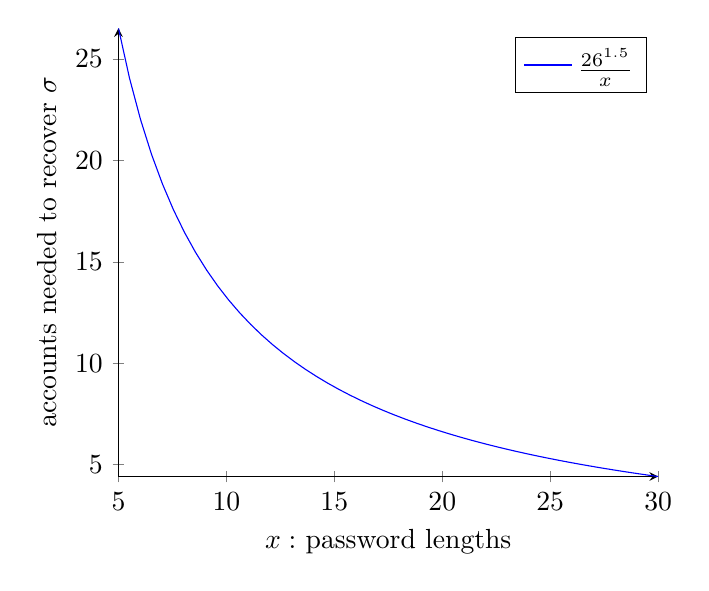
\begin{tikzpicture}
    \begin{axis}[axis lines = left, xlabel=$x: $ password lengths, ylabel=accounts needed to recover $\sigma$]
    \addplot[domain=5:30, samples=50, color=blue]{(26^1.5)/x};
    \addlegendentry{$\frac{26^{1.5}}{x}$};
\end{axis}
\end{tikzpicture}
\caption{Number of accounts needed to recover the mapping $\sigma$.}
\label{trade-off2}
\end{figure}


\begin{figure}
\begin{tikzpicture}
    \begin{axis}[axis lines = left, xlabel= Password lengths $x$, ylabel=Number of mappings $y$, ymin=0, ymax=200]
   
    \addplot+[name path=A, color=blue, domain=3:30, samples=20, no markers]{(100*x)^(2/3)};
    \addlegendentry[blue]{$100 <  \frac{y^{1.5}}{x}$};

    \addplot+[name path=B, color=red, domain=3:30, samples=20, no markers]{(50*x)^(2/3)};
    \addlegendentry[red]{$50 <  \frac{y^{1.5}}{x}$};

    \addplot+[name path=C, color=green, domain=3:30, samples=20, no markers]{(20*x)^(2/3)};
    \addlegendentry[green]{$20 <  \frac{y^{1.5}}{x}$};

    \addplot+[name path=X, domain=3:30, samples=2, no markers]{200};
    \addplot[blue!30] fill between [of=A and X];
    \addplot[red!30] fill between [of=B and A];
    \addplot[green!30] fill between [of=C and B];
\end{axis}
\end{tikzpicture}
\caption{Inequality plot of 3 different values for $\hat a$}
\label{a-var}
\end{figure}





\section{Practical Usage}\label{usage}
This section will illustrate how a human computable password scheme works in practice, using the principles described in the previous sections. Before using the scheme a user have to go through a setup procedure. \autoref{sec-params} discuss how the scheme can be tweaked to fit different needs a user may have. A summary of the setup and authentication procedures are presented next.
\subsection{Setup procedure.} \todo[inline]{setup procedure, configuration procedure, ??}
\begin{enumerate}
    \item A secret mapping is the first prerequisite required before the scheme can be used. A random mapping of length $n$ is generated from a set of objects chosen by the user, to digits in ${0,1,\dots,d}$. The user will typically chose what type of objects to use, this can be an alphabet or a user chosen set of pictures. A system will then chose $n$ of these objects and assign a random digit between $0$ and $d$, $d$ is normally $10$. 
    \item Memorization of the mapping is the next, and most costly procedure. The user basically have to learn the mappings by heart, and be comfortable he will not forget it. After memorizing, the mapping is deleted and not stored anywhere else than in the mind of the user. After finishing this step, there is no way to recover the mapping if the user forgets it. This might seem like a barrier making the scheme unusable, it will be shown later that this might not be that much of an effort after all. 
    \item Passwords can now be generated for all the accounts of the user. Algorithm \ref{new-challenge-algo} describes the process of creating a new password for an account. 
    \begin{enumerate}
        \item First the user chose the desired length of the password, $t$, to be generated. 
        \item $t$ random challenges are generated and shown one by one to the user, which calculates the responses to these. Each of the responses are one character in the new password. 
        \item The calculated password is then sent to the server which should store the salted hash of the password. In the algorithms used here, it is assumed that the sites store the password hashes properly as described in \autoref{pw-storage}. 
    \end{enumerate}
    \item the same procedure (1-3) can be done for all the accounts the user wants to include in the password scheme.
\end{enumerate}

\subsection{Authentication procedure.}\label{subsec:auth}
\begin{enumerate}
    \item Authenticating with a site, which password was previously generated using the scheme, start of by selecting the correct site. The corresponding challenges will then be displayed starting with the first one.
    \item The user calculates the response to each challenge, the same way he did when generating the password. If the calculations are done correctly, the same result should be the same password.
    \item After calculating the response to all $t$ challenges, the password can be submitted to the server which checks if the hashed value is the same as the stored one. If it is, the user is authenticated.
\end{enumerate}

\begin{remark}
    The notation $f(\sigma(\vec C))$ as used in the algorithms is equal to the composite function $f \circ \sigma(x_0,\dots,x_{13})$ as used in definition \ref{fo-function}.

\end{remark}

\begin{algorithm}
    \caption{Create new challenge for account $A_j \in (A_1,\dots, A_m)$}
    \begin{algorithmic}[1]
        \Require
            \Statex \begin{itemize}
                \item $t$ desired length of password.
                \item $\sigma$ secret mapping memorized by the user.
                \item $f$ a human computable function.
                \item $O_1,\dots,O_n$ objects, typically letters or pictures.
            \end{itemize}
            
        
        \For{$i=1 \rightarrow t$}
            \State $k \sim [0, n] $
            \State $\vec C_i \leftarrow \{O_k\}^{14} $
        \EndFor
        \Statex
        \State $\vec C \leftarrow (\vec C_1,\dots, \vec C_t) $

        \State \textbf{(User)} Computes $(p_1,\dots,p_t)=f(\sigma(\vec C))$
        \State \textbf{(Server)} Store $h_j = H(p_1,\dots,p_t)$
        \State
        \State \Return $\vec C$
    \end{algorithmic}
    \label{new-challenge-algo}
\end{algorithm}


\begin{algorithm}
    \caption{Authentication process for account $A_j \in (A_1,\dots,A_m)$}
    \begin{algorithmic}[1]
        \Require
            \Statex \begin{itemize}
                \item Account $A_j \in (A_1,\dots, A_m)$
                \item Challenges $\vec C = (\vec C_1,\dots,\vec C_t)$ from account $A_j$.
                \item Hash $h_j$ and hash function $H$.
            \end{itemize}

            \For{$i=1 \rightarrow t$}
                \State Display $C_i$ to the user
                \State \textbf{User} Compute $p_i \leftarrow f(\sigma(C_i))$
                \State
                \Comment $p_i$ is the $i$'th character of the password for account $A$
            \EndFor

            \State $\vec P = (p_1,\dots,p_t)$
            \If{$h_j =H (\vec P )$}
            \Comment \textbf{(Server)} 
                \State Authenticated on account $A_j$
            \Else 
                \State Authentication failed
            \EndIf

    \end{algorithmic}
    \label{auth-algo}
\end{algorithm}

\todo[inline]{show the procedure graphically}


\section{Usability}
Blocki et al. \cite{hcp-blocki} consider three usability parameters defining the usability of a human computable function. This section will discuss these requirements and how to influence them. 
\begin{itemize}
    \item The effort required to memorize the secret mapping.
    \item The extra rehearsal required of the user to not forget the secret mapping. 
    \item How long it takes a human user to calculate the responses to a set of challenges, eventually producing the password. 
\end{itemize}
All of these requirements might limit the usability of the scheme, and are thus worth discussing, but this project will focus mostly one the last requirement related to computation time. Later this computation time will be tested through implementing the scheme as a web app and having participants try it out will timing their efforts.

\subsection{Memorizing the secret mapping.}
As seen in the previous section, a user have to memorize a random mapping from object to digits before starting to use the scheme. This is the most likely the biggest and most frightening barrier for any user to start using the scheme. There are several techniques supposed to help us memorize relations easier, examples are the method of loci \cite{human-memory} which is supposed to enhance memory by visualization. Mnemonic helpers showing objects merged together might help memorize relations as in the case of this project. Blocki et al. \cite{hcp-blocki} propose using mnemonic helpers if the mapping consist of letters to digits. These helpers would typically be a set of pictures showing a visual transition from a letter to a digit. This way might make it easier for the user to remember it instead of only being shown "A=1" etc. Some user might also feel that it is easier to memorize other things than letters, such as pictures. The user might even get to chose the set of pictures to be used themselves as long as the corresponding digits are chosen at random. 

\subsection{Rehearsing the secret mapping.}
After memorizing the mappings the user will have to rehearse it frequent enough to not forget it. Blocki et al. \cite{naturally-rehearsing} defines a model estimating the cost of this rehearsal, the model is described in \autoref{sec:usability-model}. Applying this model to the password management scheme gives insight to how much different types of users have to rehearse their mappings. The model predicts how long a user will remember a association between $i$ and corresponding mapping $\sigma(i)$ without further rehearsing. If a user is about to forget a mapping according to the predictions he should be reminded of this. Recall \autoref{ERt} and \autoref{users} from \autoref{sec:usability-model}. The formula for $E(ER_t)$ can be used to predict how many extra rehearsals different types of users will be required to do within a given period. \autoref{extra-rehearsals} shows the expected number of extra rehearsals required by the different types of user given the length of the mapping function $n$, during the first year. It is computed using \autoref{ERt} with $t=365$ and visitation schedules $\lambda_i$ from each user type as seen in \autoref{users}. For each account $A_i$ a set of public challenges $\vec C_i \in (X_{14})^{10}$ are chosen at random using algorithm \ref{new-challenge-algo}. The expanding rehearsal assumption as defined in \cite{ER} is used, which assumes that for each rehearsal $i$ the do not have to rehearse again for $2^{is}$ units of time. The variable $i$ represents differences between user in terms of memory strength, this experiment uses $s=1$. The values in \autoref{extra-rehearsals} are calculated by generating $100$ samples of $\vec C_i \in (X_{14})^{10}$ then calculating the average expected number of extra rehearsals required by the different user types. $n$ is the number of mappings in $\sigma$.

\begin{table}
    \centering
    \begin{tabular}{ |l|c|c|c| }
        \hline
        User & $n=100$ & $n=50$ & $n=30$ \\
        \hline \hline
        Very Active & $0.396$ & $0.001$ & $\approx 0$ \\
        \hline
        Typical & $2.14$ & $0.039$ & $\approx 0$ \\
        \hline
        Occasional & $2.50$ & $0.053$ & $\approx 0 $  \\
        \hline
        Infrequent & $70.7$ & $22.3$ & $6.1$ \\
        \hline

    \end{tabular}
    \caption{\cite{hcp-blocki} Extra rehearsals required of the user during the first year to remember $\sigma$. Calculated using definition \ref{ERt} with $t=365$ and visitation schedules as in \autoref{users}.}
    \label{extra-rehearsals}
\end{table}

\par The results in \autoref{extra-rehearsals} clearly demonstrates that the human computable passwords scheme does not require much rehearsal at all if used frequently. In fact, for very active, typical and occasional users, memorizing the mapping is actually a one time cost. After memorizing the mapping at the beginning, using the scheme will provide enough natural rehearsal to maintain the mapping in memory. The simple reason for this is that for each time the user calculates the response to a challenge $\vec C$ he will have to recall 5 mappings 
When a user computes the response to a challenge $\vec C$ as described in \autoref{subsec:auth}, he will have to recall the mapping of up to $5$ ($(\sigma(x_{11}), \sigma(x_{10}), \sigma(x_{12}), \sigma(x_{13}),\sigma(x_j)$, see definition \ref{fo-function}) values of $i$ for each character of the password. A password length of $10$ would yield recalling, and thus rehearsing, $50$ values of $i$. The same trade-off as discussed in \autoref{sec-params} can be observed here. The more complex the mapping is (larger values of $n$), the more effort is required when memorizing, but no extra rehearsals are necessary even with a larger number of mappings.

\subsection{Computation Time.}
The final requirement which may limit the usability of the scheme is calculation time. If a user can not compute the response to a challenge in a reasonably short amount of time the scheme would not be usable. How much time a user can tolerate is of course individual, but a too long computation time will directly effect the usability. To make the computation as easy as possible the challenges would have to be presented to the user in a "easy to understand" fashion. Using the human computable function from definition \ref{f-function}, a challenge $C = (x_0, x_1,\dots, x_{13})$ could be displayed as shown in \autoref{challenges}. Recall the function $f(x_0,x_2,\dots,x_{13}) = x_{(x_{11} + x_{10}\quad mod \quad 10)} + x_{12} + x_{13}\quad mod \quad 10$

\begin{table}[h]
    \centering
    \begin{tabular}{|c c|c|c|}
        \hline
        $x_{10}$ & $x_{11}$ & $x_{12}$ & $x_{13}$ \\
        \hline \hline
        \multicolumn{2}{|c|}{$0:x_0$} & \multicolumn{2}{|c|}{$5:x_5$}\\
        \multicolumn{2}{|c|}{$1:x_0$} & \multicolumn{2}{|c|}{$6:x_5$}\\
        \multicolumn{2}{|c|}{$2:x_0$} & \multicolumn{2}{|c|}{$7:x_5$}\\
        \multicolumn{2}{|c|}{$3:x_0$} & \multicolumn{2}{|c|}{$8:x_5$}\\
        \multicolumn{2}{|c|}{$4:x_0$} & \multicolumn{2}{|c|}{$9:x_5$}\\
        \hline 
    \end{tabular}
    \caption{Layout template for displaying challenges.}
    \label{challenges}
\end{table}




This chapter has presented the ideas behind the human computable password management scheme. It has shown how the scheme works with a secret mapping memorized by the user and a human computable function, which together allows the user to compute passwords from challenges stored in persistent memory. Algorithms describing the procedures has been shown and described, as well as discussing the usability and security challenges of such a scheme.
